% !TEX root = ../thesis.tex
%
\chapter{Experimental Setup}%
\label{sec:experiments}

In order to compare the performance of Software Transactional Memory against Ohua in the context of shared state applications, we employ a set of benchmarks originally proposed by Minh et al.~\cite{minh2008stamp}.
In this chapter, we will categorize the benchmarks introduced by the authors and present a representative selection of applications which we will use to compare Ohua's performance against STM.
To be able to better understand the behavior of the different implementations later on, we will briefly analyze, where each application has potential for parallelization and how this could be leveraged using Ohua and STM.
Additionally, we will explain, which values we measured during execution of the benchmarks and how they are relevant for our evaluation.

\section{Benchmark Choice}
\label{sec:experiments:choice}

After presenting our transformations for Ohua in Chapter~\ref{sec:transformations}, we now wanted to compare its performance against STM in order to evaluate if Ohua could indeed be used as a suitable replacement for developing shared state applications.
To provide a comprehensive comparison, we chose to use the \emph{Stanford Transactional Applications for Multi-Processing} suite~\cite{minh2008stamp}.
Introduced by Minh et al., it was designed as a set of benchmarks for testing software transactional memory frameworks.
The authors included 8 applications from different application areas in their suite, which are supposed to resemble the diverse landscape of parallelism in applications developers might face.
In particular, the STAMP suite contains examples from different application domains and varying use cases for transactional memory such as high-contention and low-contention scenarios.

\begin{table}
    \centering
    \begin{tabular}{|l|l|l|}
        \hline
        \textbf{Application} & \textbf{Instructions per tx} \emph{(mean)} & \textbf{Time spent in transactions}\\\hline\hline
        labyrinth & 219,571 & 100\%\\\hline
        bayes & 60,584 & 83\%\\\hline
        yada & 9,795 & 100\%\\\hline
        vacation & 3,223 & 86\%\\\hline
        genome & 1,717 & 97\%\\\hline
        intruder & 330 & 33\%\\\hline
        kmeans & 117 & 7\%\\\hline
        ssca2 & 50 & 17\%\\\hline
    \end{tabular}
    \caption{A basic characterization of STAMP applications, comparing the mean number of instructions per transaction and the overall percentage of time the application spends in transactions. These numbers stem from a C implementation and have been adapted from Minh et al.~\cite{minh2008stamp}}
    \label{tab:experiments:overview}
\end{table}

The tables~\ref{tab:experiments:overview} and~\ref{tab:experiments:categorization} give a basic characterization of the benchmarks in terms of their usage of transactions.
As can be seen in table~\ref{tab:experiments:overview}, the length of individual transactions varies greatly per application, as does the overall time that is spent by the benchmark executing transactions.
Even though the numbers in the table have been adapted from Minh et al.\ and represent values measured for their C-based implementation, they still outline the general characteristics of the respective STM-based algorithms.
Some applications suffer so badly from the irregular properties outlined in Chapter~\ref{sec:background:irregular} that exploiting their parallelism requires them to spend more than 80 \% of their overall execution time in transactions.
This is for example the case in the \emph{labyrinth} benchmark, where fields of a dense 3-dimensional matrix have to be continuously updated, as we explained in Chapter~\ref{sec:preliminary:labyrinth}.
Other applications such as \emph{kmeans} or \emph{ssca2} have relatively short transactions, meaning their data parallelism is easier to exploit or they generally do not feature as much opportunities for parallelism as other applications.

\begin{table}
    \centering
    \begin{tabular}{|l|l|l|l|l|}
        \hline
        \textbf{Application} & \textbf{tx length} & \textbf{r/w set} & \textbf{tx time} & \textbf{Contention}\\\hline\hline
        labyrinth & long & large & high & high\\\hline
        bayes & long & large & high & high\\\hline
        yada & long & large & high & medium\\\hline
        vacation & medium & medium & high & low/medium\\\hline
        genome & medium & medium & high & low\\\hline
        intruder & short & medium & medium & high\\\hline
        kmeans & short & small & low & low\\\hline
        ssca2 & short & small & low & low\\\hline
    \end{tabular}
    \caption{A qualitative summary of each STAMP application's runtime transactional characteristics. The length of a transaction is determined by the number of instructions it encompasses. The characteristics are ranked relative to the other applications in the suite. Adapted from Minh et al.~\cite{minh2008stamp}}
    \label{tab:experiments:categorization}
\end{table}

Another relevant and perhaps the most limiting factor for programs relying on optimistic parallelism principles such as STM is contention.
This characteristic is visualized in table~\ref{tab:experiments:categorization} along with other properties.
When facing high contention scenarios, STM implementations are usually unable to achieve the near-linear speedups Minh et al.\ reported for other benchmarks.
Contention is a byproduct of frequent reading and writing accesses to the shared data structure that inevitably lead to frequent conflicts which require a rollback of all affected transactions except for the one that committed its changes first.
Hence, the relative amount of reads and writes per transaction is also reported in table~\ref{tab:experiments:categorization}.
Long transactions, large read/write sets, more time spent in transactions and high contention are all factors promoting conflicts.
The results of conflicts are frequent rollbacks and accompanying recomputations, which reduce the overall performance.

Based on the analysis provided by the authors, we selected a representative range of benchmarks for our comparison between Ohua and STM.
We chose applications with varying transaction lengths and frequency of transaction use as well as different levels of contention.
The next sections will briefly outline the details of the chosen benchmarks and explain, how they were implemented.


% THEN elaborate further about the technical details that hold true for all benchmarks
Since the authors only provided a C-based reference implementation for their programs, we had to re-implement them in Rust to rule out language-specific performance changes when comparing to Ohua's Rust implementation.
We chose to use the \texttt{rust-stm} library written by Bergmann et al.~\cite{bergmann2020stm} for these implementations.
Upon inspecting the original source code, it turned out that the authors adapted the code in order to improve the performance of STM in some benchmarks.
For instance, they provided their own implementation of a \rust{HashMap}\footnote{A dynamic key-value store allowing fast lookups by hashing the keys and organizing them in different buckets.} that offered the use of transactions on a per-bucket basis, effectively exposing fine-granular parallelization opportunities that normal HashMaps cannot provide.
In Rust, no corresponding STM-specific data structures existed prior to this work.
We debated, whether or not we should use these optimizations in our own implementation but ultimately decided in favor of doing so.
First, one could argue that these optimizations would be made by developers anyway after deciding to use the STM framework in an attempt to tailor the program code towards the library used.
Secondly, we wanted to remain as close as possible to the original implementations from Minh et al.\ in the hopes of achieving similar results for STM as they did.
Therefore, we contributed a small library~\cite{wittwer2020stmdata} which provides data structures like HashMaps and HashSets augmented for the use with transactions.
Both the library and the benchmarks were implemented from scratch based on the descriptions provided by the authors, literature they cited and the code they supplied.
We did so in an idiomatic way, applying both concepts to the problems using the tools the frameworks and the STM data structure library provide natively.
As implementing the Ohua transformations proposed in Chapter~\ref{sec:transformations} has been left for future work, we applied these transformations manually to the algorithms.
The code for all benchmarks we wrote for this thesis may be found online~\cite{wittwer2020benchmarks}.

When implementing the \emph{labyrinth} benchmark, we found that two transactions may deadlock.
We have reported this issue~\cite{wittwer2020stmissue} and resorted to forking and patching the library~\cite{wittwer2020stm} in question to move on with our tests.


\subsection{Parallelism Opportunities}
\label{sec:experiments:opportunities}

When presenting each benchmark, we will provide a short assessment of the opportunities for parallelism it provides and how they can be exploited when using Ohua and STM.
Goal of this analysis is to detect structural limitations within the benchmarks which one of the frameworks cannot overcome to exploit the full available parallelism.
For this analysis, we produced an abstract prepresentation of each selected application which aims to point out a program's structural parallelism opportunities.
To keep this representation concise and simple, we simplified each algorithm by removing loop conditions, abort conditions and any unnecessary computations.
The resulting abstracted code snippets only contain the main operations performed on the input data to produce the end result as well as any shared state used.


\subsection{Labyrinth Path Mapping}
\label{sec:experiments:labyrinth}

The labyrinth benchmark we presented in Chapter~\ref{sec:preliminary:labyrinth} based on the work of Swalens et al.~\cite{swalens2016transactional} was originally proposed by Minh et al. as possible benchmark for Software Transactional Memory.
Since we have already analyzed and implemented this application, it was apparent for us to adduce it for our concluding comparison.
Additionally, it is one of few benchmarks in the suite exhibiting amorphous data parallelism, a trait the authors did not consider when compiling their benchmark list but which they happened to include by coincidence, as it is frequently encountered in real-life applications using shared state, the main use case for transactional memory applications.
Another interesting property of the benchmark was its frequent use of transactions (the whole algorithm is executed within transactions) and the high contention on the shared data structure, which puts the synchronization primitives under heavy stress, as described before.

\begin{listing}
    \begin{minted}[fontsize=\footnotesize]{Rust}
        let mut maze = Maze::initialize();
        for pair in points {
            let path = find_path(maze, pair);
            maze.update(path);
        }
    \end{minted}
    \caption{Abstract description of the \emph{labyrinth} algorithm}
    \label{fig:experiments:opportunities:algos:labyrinth}
\end{listing}

As can be seen in Listing~\ref{fig:experiments:opportunities:algos:labyrinth}, the \emph{labyrinth} application consists of a state-modifying loop.
After finding a path for each input coordinate pair, the maze gets updated accordingly.
This intertwining of calculation and state update is customary to programs exhibiting amorphous data parallelism, as it creates these dependencies between separate calculations in the first place.
When using STM for concurrency control, one can execute the whole loop in parallel, guarding each individual iteration using a transaction, resulting in the 100 \% transaction coverage reported in Table~\ref{tab:experiments:overview}.
Ohua is also able to exploit the parallelism in this loop due to the Transformations~2 and~3, allowing both approaches to possibly exploit the maximal available parallelism.

\subsection{Intruder Detection}
\label{sec:experiments:intruder}

The intruder application implements a signature-based Network Intrusion Detection System (NIDS) and is used in networking to detect attacks or malicious activities in an active network as well as policy violations.
It is based on design proposal number five of Haagdorens et al.'s work on \enquote{Improving the Performance of Signature-Based Network Intrusion Detection Sensors by Multi-Threading}~\cite{haagdorens2004improving}.

The basic function of this application is to scan incoming network packets and match them against known intrusion signatures.
This happens in three distinct stages, as outlined in Fig.~\ref{fig:experiments:intruder:workflow}.
Incoming network traffic is captured and queued for inspection.
Due to the architecture of modern network protocols, individual data flows have to be split into several packets that are transmitted individually and may reach the recipient out of order.
Attackers have used this in the past by splitting malicious flows and sending them out of order to avoid detection.
To counter this, the second step in the algorithm is to deploy stateful detection avoidance countermeasures, which involve preprocessing the received packets and reassembling the original flows.
These flows can then finally be matched against known attack patterns, filtering any malicious packets from the stream of incoming data.

\begin{figure}
    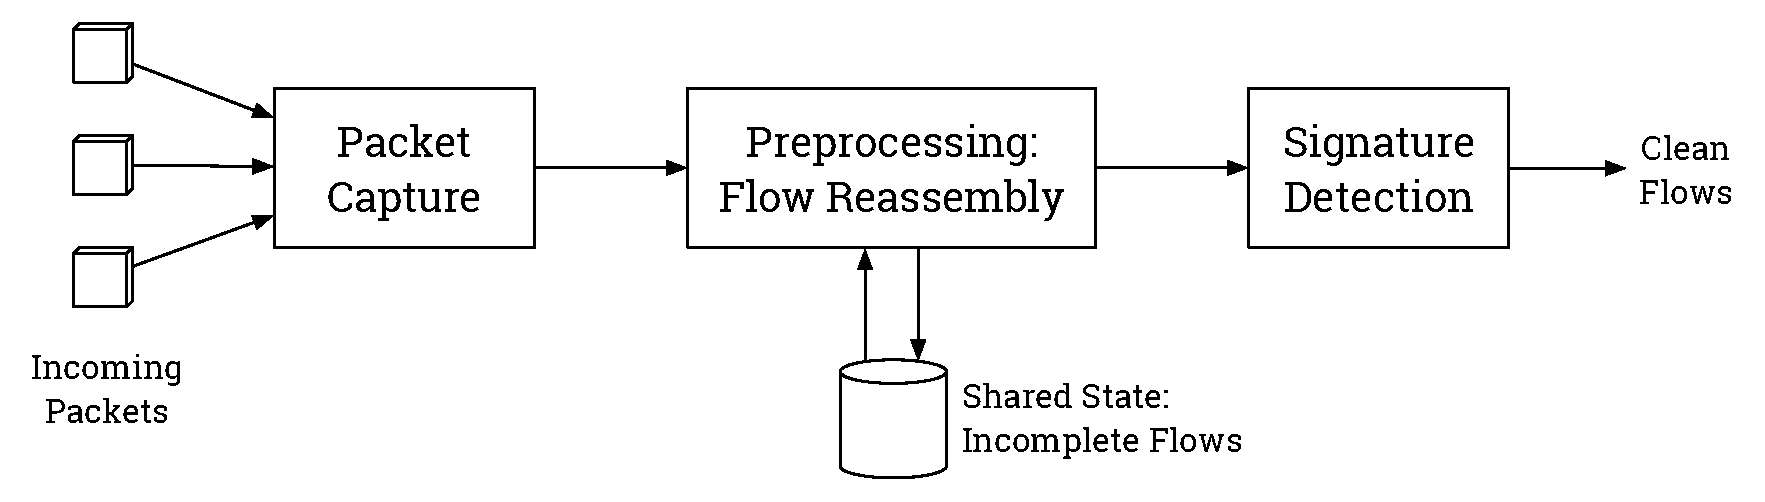
\includegraphics[width=\textwidth,keepaspectratio]{gfx/experiments-intruder}
    \caption{Workflow of the \emph{intruder} benchmark. Processing of incoming data is conducted in three stages.}%
    \label{fig:experiments:intruder:workflow}
\end{figure}

\begin{listing}
    \begin{minted}[fontsize=\footnotesize]{Rust}
        let mut flows = State::new();
        for packet in input {
            flows.add(packet);
        }

        for flow in flows {
            analyze(flow);
        }
    \end{minted}
    \caption{Abstract description of the \emph{intruder} algorithm}
    \label{fig:experiments:opportunities:algos:intruder}
\end{listing}

In this application, no amorphous data parallelism may be found.
Instead, we encounter two loops of which one is stateful and the other state-free, as shown in Listing~\ref{fig:experiments:opportunities:algos:intruder}.
The flow reassembly phase (step two) happens in parallel in the STM implementation, using a transaction-aware HashMap.
Since the loop body does not contain any other state-free functions, there are no parallelization opportunities for Ohua as no transformations from Chapter~\ref{sec:transformations} are applicable.
Also, it would not make sense to attempt to exploit parallelism from this loop using any workarounds, so it is executed sequentially.
This shows that Ohua may only extract non-trivial parallelism from irregular applications that fit certain criteria, i.e., contain loops that do not solely consist of state-modifying operations, as its main approach is to exploit data parallelism by the use of certain transformations to uncover it.
Both approaches manage to implement the state-free analysis loop (step three) in parallel as again no concurrency control is necessary.
Ohua does this using Transformations~1 and~4.
Our evaluation will show, if it is more performant to attempt exploiting parallelism from the stateful loop or if a sequential approach as done in Ohua performs better.

This benchmark was chosen because it is mostly similar in its properties to the labyrinth application as it also features short transactions and high contention on the shared data, but does only spend about 33 \% of the overall execution time in transactions.
We mainly wanted to see, how this slight difference in properties is reflected in the performance results.


\subsection{K-means Clustering}
\label{sec:experiments:kmeans}

Proposed as benchmark by Narayanan et al.~\cite{narayanan2006minebench} the k-means clustering algorithm partitions a set of $n$ observations into $k$ clusters.
It was originally put forth by MacQueen et al. in 1967~\cite{macqueen1967some} and still is a very popular algorithm for cluster analysis in data mining which is often used to classify data.

The inner workings of the algorithm are rather simple: It takes a set of $n$ observations and a desired number of clusters to sort the observations into.
Then the $k$ cluster centroids are initialized.
Many ways exist to realize this but we chose, akin to our C reference implementation, to select the coordinates for each cluster centroid randomly from the coordinates preset by the input data set.
Following this initialization, each observation is assigned to its nearest cluster based on the squared multi-dimensional spatial euclidian distance between both points.
Afterwards, new centroids are computed by calculating the means of all observations now assigned to a certain cluster.
These last two steps now get repeated iteratively until the algorithm either reaches an upper bound of iterations or converges, i.e., less than a certain percentage of observations change per iteration.

\begin{listing}
    \begin{minted}[fontsize=\footnotesize]{Rust}
        let mut centers = initialize(input);
        loop {
            // data parallelism
            for item in input {
                item.find_center(centers);
            }
            // fold
            centers = recompute(input);
        }
    \end{minted}
    \caption{Abstract description of the \emph{kmeans} algorithm}
    \label{fig:experiments:opportunities:algos:kmeans}
\end{listing}

In the \emph{kmeans} application, all parallelizable calculations happen within the single state-free innermost loop, which assigns all observations to a new centroid before the new centroids are calculated sequentially.
This is shown in Listing~\ref{fig:experiments:opportunities:algos:kmeans}.
The STM implementation introduces some shared state for deciding on the convergence of the algorithm (not depicted in the abstract representation) and for updating the centroids during the inner loop iteration, executing the whole body of the outermost loop in parallel using transactions.
Ohua exploits the data parallelism of the inner loop using Transformations~1 and~4 to exploit data parallelism.
As both approaches are able to exploit all opportunities for parallelism, though each does it differently, we expect similar performances for both implementations.

k-means is very much like the intruder benchmark in the regard that its parallelism opportunities are limited to a single state-free loop but unlike the aforementioned benchmark k-means features low contention on shared data structures while presenting a similar transaction utilization, making this an interesting benchmark to look at.

\subsection{Genome Sequencing}
\label{sec:experiments:genome}
This benchmark implements a \emph{\enquote{whole-genome shotgun sequencing}} algorithm as outlined by Pop et al.~\cite{pop2002genome} in their work.
Its goal is to sequence a (fictional) genome, i.e.\ to reassemble a nucleotide sequence from a set of snippets which is something frequently done in genetics.

\begin{figure}
    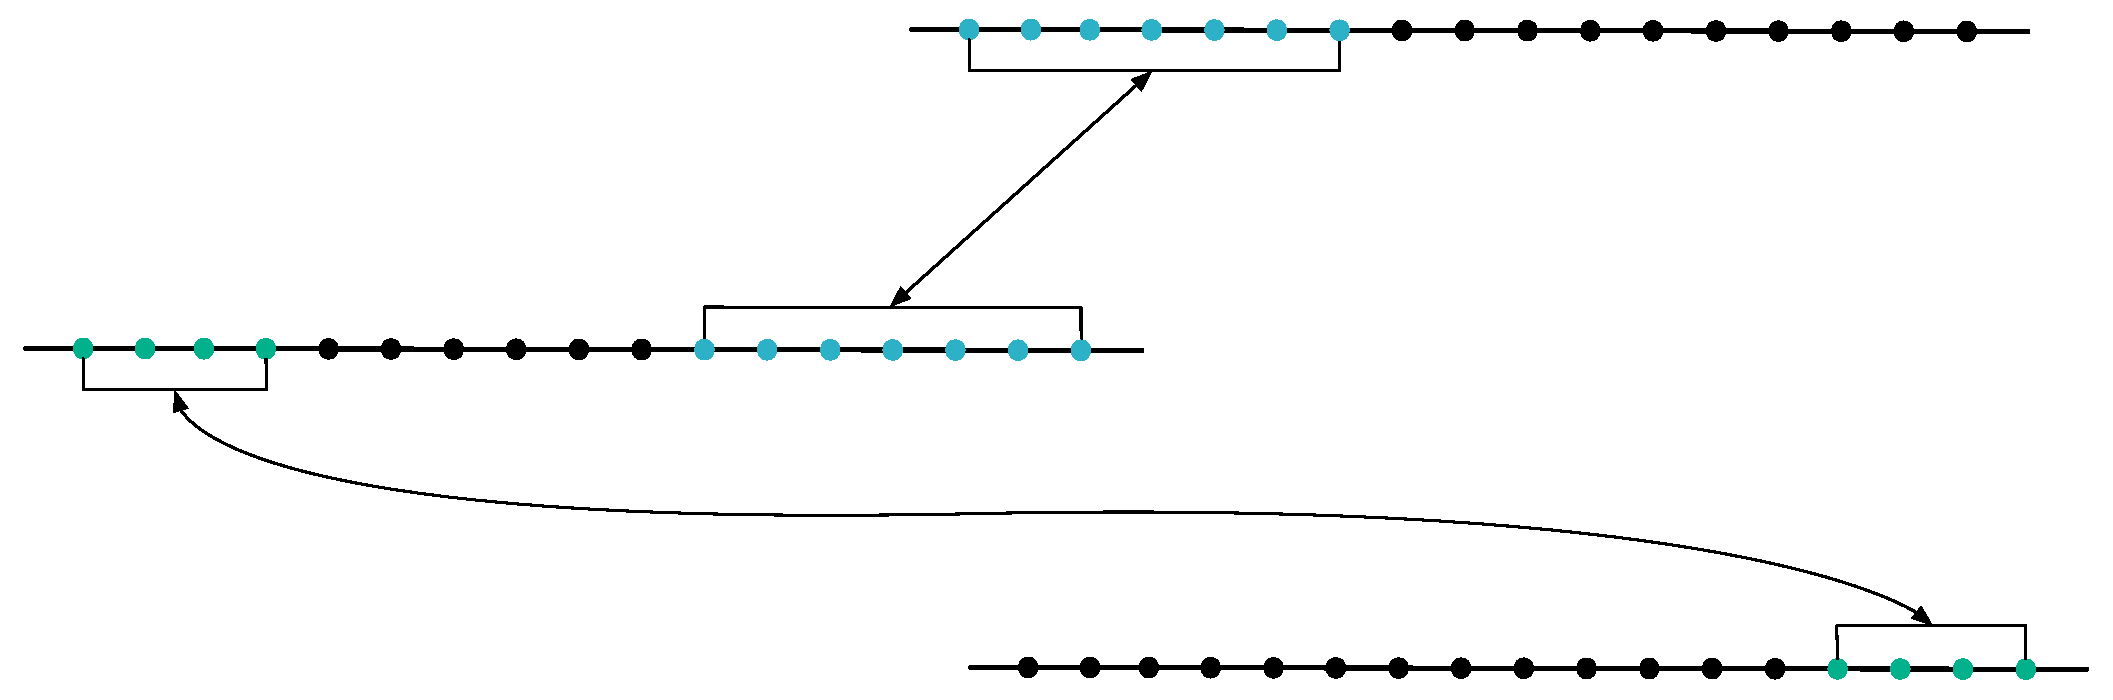
\includegraphics[width=\textwidth,keepaspectratio]{gfx/experiments-genome}
    \caption{Visualization of the overlap matching found in the \emph{genome} benchmark. The blue match is stronger as it has seven matching elements and has hence been found first.}
    \label{fig:experiments:genome-example}
\end{figure}

The first step in the algorithm is to deduplicate the DNA segments that have been provided as inputs, since there are usually many duplications.
The second phase is then concerned with finding neighboring segments in the remaining pool of DNA parts by utilizing overlap matching.
By reducing the overlap size each iteration, the best possible fit is chosen for each neighbor search.
Figure~\ref{fig:experiments:genome-example} provides visualization of how this matching works.
Starting from a match length of $n-1$, the algorithm attempts to find a matching predecessor-successor pair for all loose ends.
With each iteration, the match length is reduced, until it ends with an overlap of one.
In our example, the blue overlap match is found first due to seven matching nucleotides.
Three iterations later, the green match is established, fully connecting the centered genome segment.
After this phase has finished, all but two segments have a predecessor and successor assigned.
Starting from the one element in the set with no predecessor, the chain of nucleotides can be rebuilt by simply following the links.

\begin{listing}
    \begin{minted}[fontsize=\footnotesize]{Rust}
        let mut nucleotides = Hashset::new();
        for segment in input {
            // deduplication
            nucleotides.insert(segment);
        }

        loop {
            for item in nucleotides {
                item.find_neighbor(nucleotides);
            }
        }
    \end{minted}
    \caption{Abstract description of the \emph{genome} algorithm}
    \label{fig:experiments:opportunities:algos:genome}
\end{listing}

\emph{genome} consists, as outlined in Listing~\ref{fig:experiments:opportunities:algos:genome}, mainly of two separate loops.
The first loop expression to deduplicate the input set is again a purely state-modifying loop, as seen before in the \emph{intruder} benchmark.
All operations in the loop body are directly accessing the shared state, making parallelization difficult.
The second loop on the other hand is state-free, allowing for the simple exploiting of the parallelism within without the need for concurrency control.\\
Providing a parallel implementation for the first loop however, is more challenging.
Only by using a transaction-aware HashMap with $k$ buckets, the STM implementation is able to exploit the loop's parallelism for up to $k$ conflict-free accesses.
Ohua, again unable to use any transformations for leveraging parallelism, may also exploit a certain part of parallelism by emulating the same behavior as STM and partitioning the input set beforehand into $k$ parts, so that the compiler may break the resulting state-free loop using the first transformation:
\begin{minted}{Rust}
fn dedup(segments: Segments, threadcount: usize) -> Vec<SequencerItem> {
    let parts = partition(segments, threadcount);
    for p in parts {
        deduplicate(p)
    }
}
\end{minted}
This application example shows, that even when using Ohua, code sometimes has to be written in a certain way to expose the parallelism opportunities of a computation to the compiler.
Nevertheless, the resulting Ohua algorithms can still be executed as a sequential program while the resulting STM code, which is even more optimized by the use of special data structures, is unable to do so.
Overall, we expect differing results for both implementations, as they try to exploit the parallelism hidden in the first stateful loop in different ways, probably with varying degrees of success.

All in all we chose this application to complete our benchmark selection as it provides similar properties as the kmeans benchmark in terms of transaction length and contention but spends nearly all its execution time in transactions, a stark change compared to the 7 \% of transaction time in kmeans.

\subsection{Summary}
\label{sec:experiments:opportunity-summary}

In summary, we found in our analysis that only the labyrinth application contains amorphous data parallelism and is the only application where Ohua's Transformations~2 and~3 are applicable.
All other benchmarks contain loops that are state-free, while possibly occuring state modifications exist in separate loops.
While STM can be used to exploit parallelism from the latter, Ohua has to execute this type of loop sequentially to avoid handling shared state.
Therefore, we expect to see different behavior in the labyrinth application than in the other applications for Ohua's performance compared to STM.

\section{Reference Measurements}
\label{sec:experiments:reference}

Minh et al.\ proposed their STAMP suite in 2008.
Since then, hardware (e.g., clock speeds of CPUs) as well as compile-time optimizations have evolved significantly, rendering the results provided in their paper outdated.
Hence, we decided to run the benchmarks relevant to our investigation again, on the same hardware and under the same conditions as our Rust benchmarks to have a reference we can compare our STM implementations to.
Although the authors themselves only measured results for the smaller two of their three suggested input sets, we tested all three to have a more comprehensive set of results to compare our STM implementation against.

Upon building and executing the benchmarks with the included \texttt{tl2} STM implementation~\cite{minh2013stampcode}, a number of issues with the STAMP suite became apparent, which we already briefly touched upon in Chapter~\ref{sec:introduction}.
The genome benchmark could not be built from the original source code, due to conflicts caused by compile-time memory allocation patching.
We reported this issue~\cite{wittwer2020stampgenome} and employed a workaround to be able to use the benchmark nonetheless.
Additionally, we found that the implementation of the labyrinth benchmark sometimes does not yield a correct solution, causing the program to crash~\cite{wittwer2020labyrinth}.
Similar behavior was found for the intruder application, although we did not investigate this further, instead discarding failed runs in both cases, lowering the effective number of test results slightly below 30.
These issues cement some of the drawbacks of STAMP and STM in general, which we discussed in the beginning of this thesis.

For comparability and in order to provide a more complete performance graph, we intended to run the selected four benchmarks for the same range of threads as our own applications but the suite only supports thread counts which are a power of two, leaving us with 1, 2, 4, 8 and 16 threads as test parameters.
Due to this limited result range, we will only be able to draw vague general comparisons between STAMPs STM and our own STM implementation as the sparse result coverage for higher thread counts leaves us unable to reliably identify trends in the performance of STAMP.

\section{Measurements}
\label{sec:experiments:measurements}

In our experiments, we tried to achieve reproducible and plausible results so that we can make an educated comparison between both STM and Ohua.
This section will briefly explain our benchmarking setup to enable others to reproduce our results.

\subsection{Input Data}
\label{sec:experiments:measurements:inputs}

For each STAMP application, Minh et al.~\cite{minh2008stamp} additionally provided three sets of parameters to model small, medium and large workloads.
We adopted these parameters with only minor modifications, as intended by the authors.
A change was made to the parameters of the \emph{genome} benchmark as the input data that was randomly created using the original input parameters proved faulty in our re-implementation.
Also, a unnecessary parameter was removed from the \emph{kmeans} benchmark.

\begin{table}
    \centering
    \tiny
    \begin{tabular}{|l l l|}
        \hline
        \textbf{Application} & \textbf{Arguments} & \textbf{Description}\\\hline\hline
        genome & -g 256 -s 16 -n 16384 & \multirow{3}{*}{\begin{minipage}{.4\textwidth}$n$ gene segments of length $s$ are first sampled from a gene consisting of $g$ nucleotides and then reassembled again.\end{minipage}}\\
        genome+ & -g 510 -s 32 -n 32768 & \\
        genome++ & -g 16384 -s 64 -n 16777216 & \\\hline

        intruder & -a 10 -l 4 -n 2048 -s 1 & \multirow{3}{*}{\begin{minipage}{.4\textwidth}From seed $s$, $n$ traffic flows are generated, $a\%$ of which contain attacks. Each flow consists of up to $l$ packets, which are assembled and inspected by the program.\end{minipage}}\\
        intruder+ & -a 10 -l 16 -n 4096 -s 1 & \\
        intruder++ & -a 10 -l 128 -n 262144 -s 1 & \\\hline

        kmeans-high & -n 15 -t 0.05 -i random-n2048-d16-c16.txt & \multirow{6}{*}{\begin{minipage}{.4\textwidth}The input file $i$ containing $n$ points in $d$ dimensions generated about $c$ centers is loaded and then clustered into $n$ clusters. A convergence threshold of $t$ is used.\end{minipage}}\\
        kmeans-high+ & -n 15 -t 0.05 -i random-n16384-d24-c16.txt & \\
        kmeans-high++ & -n 15 -t 0.00001 -i random-n65536-d32-c16.txt & \\
        kmeans-low & -n 40 -t 0.05 -i random-n2048-d16-c16.txt & \\
        kmeans-low+ & -n 40 -t 0.05 -i random-n16384-d24-c16.txt & \\
        kmeans-low++ & -n 40 -t 0.00001 -i random-n65536-d32-c16.txt & \\\hline

        labyrinth & -i random-x32-y32-z3-n96.txt & \multirow{3}{*}{\begin{minipage}{.4\textwidth}The input file $i$ describes a maze of dimensions $x \times y \times z$ and $n$ paths to map.\end{minipage}}\\
        labyrinth+ & -i random-x48-y48-z3-n64.txt & \\
        labyrinth++ & -i random-x512-y512-z7-n512.txt & \\\hline
    \end{tabular}

    \caption{Input data sets for the benchmarks presented in this thesis. Adapted from Minh et al.~\cite{minh2008stamp} and adjusted to mitigate flaws in the original algorithms.}
    \label{tab:experiments:inputs}
\end{table}

Table~\ref{tab:experiments:inputs} gives a full overview over all parameters we used.
Input sets marked with a + indicate a larger input and an appended ++ marks the largest of the three input sets for a benchmark.
The \emph{kmeans} benchmark inputs are additionally labeled as \emph{high} and \emph{low}, which refers to the relative amount of contention produced by the inputs.

\subsection{Measured Values}
\label{sec:experiments:measurements:values}

For the purpose of our comparison between Ohua and STM, two values are of importance and have hence been measured.
As we are calculating the speedups of both implementations in reference to a sequential implementation, the execution time in milliseconds, i.e., the time it takes the algorithm to complete, is relevant.
Moreover, we were interested in the power consumption of both algorithms.
But since measuring the power consumption of the algorithms would have been to complicated and time-consuming, we opted for measuring the total CPU time used by the programs, as the amount of power used while processing is resulting from the utilization of a PCs individual components.
Since all these programs are performing purely in-memory computations, we figured that measuring the CPU time would be a sufficient approximation to draw some general conclusions regarding the power usage.

For both measured values, the setup phase (parsing input arguments and reading input files) and teardown phase (writing the results to a file) where not included in the measurements.
This was done in order to reduce potential noise from Operating System calls resulting from the I/O operations performed in these stages.
Research has shown in the past that this noise, as well as different contention scenarios can severely impact the measured time values, leading to variations in the measured time values.
To take this into account and produce more realistic results, each measurement has been done 30 times, so that statistical outliers do not carry as much weight.
From the resulting measured values the geometric mean was calculated per data point to compile all measurements into a single data point.

Using the measured execution times in Milliseconds, we calculated the speedup using the following equation:
\[
    S_c = \frac{t_{seq}}{t_f}
\]
where $S_c$ is the speedup of the configuration under investigation, $t_{seq}$ is the mean execution time of the sequential implementation and $t_f$ the mean execution time of the framework in question.

\subsection{Running Configuration}
\label{sec:experiments:measurements:hardware}

All benchmarks conducted for this work were run on an Ubuntu 18.04 server with 128GB RAM and two Intel Xeon E5-2630 v2 processors which have a base frequency of 2.60 GHz and offer combined 12 cores with 24 threads.
At all times, the program under inspection was running exclusively on the machine, meaning that aside from background operating system jobs, no other tasks ran on the system simultaneously.


